\section{The $\pvslm$ Description Language}
\label{sec.conf}

\begin{table*}[pthb]
  \centering
  \begin{tabular}{r c p{8cm}}
    \hline \\
    $\nterm{\cde{metadata}}$ & ::= & $\nterm{\cde{header}} \; \nterm{\cde{body}}$ \\
    $\nterm{\cde{header}}$ & ::= & `/' $\nterm{\cde{theorylist}}$ \\
    $\nterm{\cde{theorylist}}$ & ::= & $\nterm{\cde{theory}} \mid \nterm{\cde{theory}}$ `,' $\nterm{\cde{theorylist}}$ \\
    $\nterm{\cde{body}}$ & ::= & $(\nterm{\cde{packagedep}} \mid \nterm{\cde{theorydep}})*$ \\
    $\nterm{\cde{packagedep}}$ & ::= & $\nterm{\cde{package}}$ `/' $\nterm{\cde{theorylist}}$ \\
    $\nterm{\cde{theorydep}}$ & ::= & $\nterm{\cde{theory}}$ `:' $\nterm{\cde{qualtheorylist}} ?$ \\
    $\nterm{\cde{qualtheorylist}}$ & ::= & $\nterm{\cde{qualtheory}} \mid \nterm{\cde{qualtheory}}$ `,' $\nterm{\cde{qualtheorylist}}$ \\
    $\nterm{\cde{qualtheory}}$ & ::= & $(\nterm{\cde{package}}\; \text{`@'})?$ $\nterm{\cde{theory}}$ \\
    \\
    \hline
  \end{tabular}
  \caption{Syntax of the \cde{top.dep} metadata file in NASALib.}
  \label{tab.bnf}
\end{table*}

This section presents a formal definition of the $\pvslm$ description
language in the form of BNF-like notation, adopted from the NASA PVS
library. It also presents the main conventions and assumptions used by
the $\pvslm$ tool for managing PVS libraries. It is important to point
out that the description language was first proposed by the NASA
Langley Formal Methods Team for documenting its NASA PVS library: the
main contribution of this paper, in this regard, is the formal
formulation of such a description language.

\paragraph{Terminology}
The $\pvslm$ tool distinguishes three levels of aggregation for PVS
sources. A PVS theory is the building block of a library managed by
$\pvslm$. A {\em package} is a collection of theories.  A {\em
  library} is at the top level of aggregation, comprising a collection
of packages. In summary, a library is a collection of packages and a
package is a collection of theories. The $\pvslm$ tool can manage
several libraries each with several packages.

\paragraph{Package configuration}
A package is defined in a folder at the root of the library source,
with the folder name defining the name of the package. Each folder
contains the \cde{pvs} and \cde{prf} files for its theories, and a
folder named \cde{pvsbin}: this is a special folder used by the
$\pvslm$ implementation for accessing the {\em package metadata} from
a file named \cde{top.dep}.

\paragraph{Package metadata} The metadata of a package is defined
in its \cde{top.dep} file, located inside folder
\cde{pvsbin}. Table~\ref{tab.bnf} presents the syntax of $\pvslm$
description language, in BNF-like notation, used to populate this
metadata file.

The topmost symbol in the description language is
$\nterm{\cde{metadata}}$, while $\nterm{\cde{theory}}$ and
$\nterm{\cde{package}}$ are terminals representing, respectively,
theory and package names. The metadata comprises two parts, namely, a
header and a body. The header corresponds to a single line with an `/'
symbol followed by a comma-separated list of theory names; these names
correspond to the names of the theories included in the package (in
any order). A body comprises any number of lines, each with either a
package dependency or a theory dependency. A package dependency
describes a dependency from another package and the list of theories
from that package that are being depended upon. A theory dependency
describes, for each one of the theories listed in the header of the
package, the list of its theory dependencies. In the case such a
theory depends on a theory from other package, the name of that
dependency must be qualified by the name of its package.

Figure~\ref{fig.top} presents an overview of the configuration file
for package \cde{trig} in NASALib. According to its header
description, package \cde{trig} defines theories \cde{top},
\cde{trig\_doc}, \cde{trig}, \cde{trig\_values}, etc. It contains $5$
package dependencies and $6$ theory dependencies. For instance,
package \cde{trig} depends on theory \cde{for\_iterate} in package
\cde{structures}, and on theories \cde{finite\_sets\_minmax} and
\cde{finite\_sets\_inductions} in package \cde{finite\_sets}. On the
other hand, theory \cde{trig\_doc} has no dependencies, while theory
\cde{trig} depends on theories \cde{trig\_basic}, \cde{sqrt},
\cde{trig\_values}, and \cde{trig\_ineq}. In the case of theory
\cde{sqrt}, it is explicitly stated that such a theory is in package
\cde{reals}.

\begin{figure*}[pthb]
  \centering
  \begin{minipage}[c]{0.8\textwidth}%
	\begin{center}
    \input{top.dep.txt}
  %  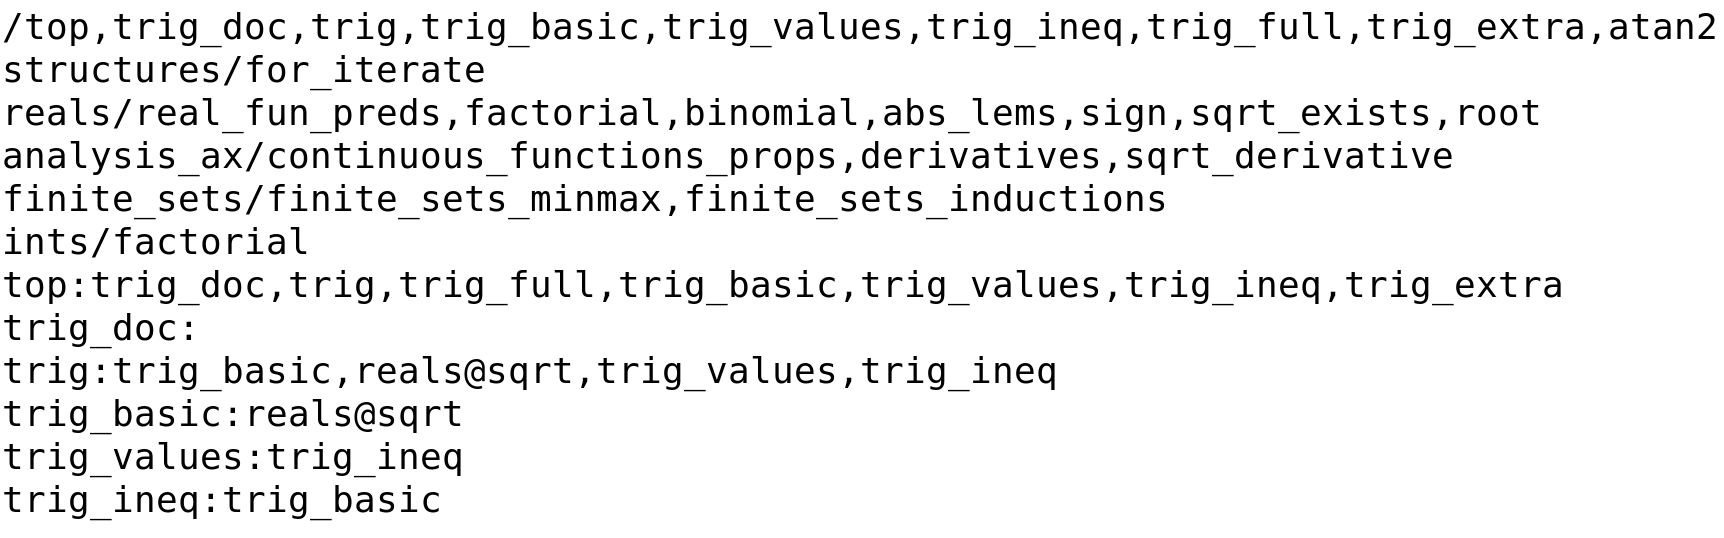
\includegraphics[width=12cm]{images/top.png}
  \end{center}
\end{minipage}
  \caption{Overview of metadata file for package \cde{trig} in NASALib.}
  \label{fig.top}
\end{figure*}
